\chapter{Specifikacija programske potpore}
		
	\section{Funkcionalni zahtjevi}
			
			\textbf{\textit{dio 1. revizije}}\\
			
			\textit{Navesti \textbf{dionike} koji imaju \textbf{interes u ovom sustavu} ili  \textbf{su nositelji odgovornosti}. To su prije svega korisnici, ali i administratori sustava, naručitelji, razvojni tim.}\\
				
			\textit{Navesti \textbf{aktore} koji izravno \textbf{koriste} ili \textbf{komuniciraju sa sustavom}. Oni mogu imati inicijatorsku ulogu, tj. započinju određene procese u sustavu ili samo sudioničku ulogu, tj. obavljaju određeni posao. Za svakog aktora navesti funkcionalne zahtjeve koji se na njega odnose.}\\
			
			
			\noindent \textbf{Dionici:}
			
			\begin{packed_enum}
				
				\item Razvojni tim
				\item Igrači				
				\item Kartografi
				\item Admin
				
			\end{packed_enum}
			
			\noindent \textbf{Aktori i njihovi funkcionalni zahtjevi:}
			
			
			\begin{packed_enum}
				\item  \underbar{Neregistrirani korisnik (inicijator) može:}
				
				\begin{packed_enum}
					
					\item se registrirati u sustav kao:
					\begin{packed_enum}
						
						\item  igrač (stvaranje korisničkog računa, potrebni sljedeći podaci: korisničko ime, lozinka, e-mail adresa, fotografija)
						\item  kartograf (stvaranje korisničkog računa, potrebni sljedeći podaci: IBAN računa za uplatu, fotografija osobne iskaznice)
				
					\end{packed_enum}
					
				\end{packed_enum}
			
				\item  \underbar{Igrač (inicijator) može:}
				
				\begin{packed_enum}
					
					\item se prijaviti u sustav koristeći email i lozinku
					\item se odjaviti iz sustava
					\item pregledati vlastiti profil
					\begin{packed_enum}
						\item pristupiti prikazu svih sakupljenih karti
						\item pristupiti prikazu statistike 10 zadnjih odigranih borbi
					\end{packed_enum}
				\item pregledati profil drugog igrača
				\begin{packed_enum}
					\item pristupiti prikazu svih sakupljenih karti
					\item pristupiti prikazu statistike 10 zadnjih odigranih borbi
				\end{packed_enum}
			\item pregledati detalje pojedinačne karte iz kolekcije
			\item pregledati popis igrača u blizini
			\item pristupiti borbi kroz nasumičnu tražilicu
			\item se boriti u kartaškom dvoboju protiv drugog igrača
			\begin{packed_enum}
				\item odabrati karte za borbu iz svoje kolekcije sakupljenih karata
				\item odigrati kartaški dvoboj
			\end{packed_enum}
		\item prijaviti novu lokaciju
		\item dobiti novu kartu ako ju je igrač prijavio te je ona odobrena bez izmjena
		\item pristupiti pregledu rang ljestvice svih igrača
					
				\end{packed_enum}
			\item  \underbar{Kartograf (inicijator) može:}
			
			\begin{packed_enum}
				\item se prijaviti u sustav preko broja osobne iskaznice
				\item se odjaviti iz sustava
				\item pristupiti prikazu svih prijava:
				\begin{packed_enum}
					\item prihvatiti lokaciju iz prijave
					\item odbiti lokaciju iz prijave
					\item može izmijeniti prijavu te zatim lokaciju prihvatiti
					\item može odabrati opciju da je potrebna potvrda s terena, te ga sustav na mapi vodi najkraćim putem od vlastite lokacije do prijavljene lokacije
				\end{packed_enum}
			\end{packed_enum}
		\item  \underbar{Administrator (inicijator) uz mogućnosti kartografa i igrača može:}
		\begin{packed_enum}
			\item pristupiti pregledu popisa svih korisnika
			\begin{packed_enum}
				\item brisati korisnike s popisa, odnosno ukloniti korisnike iz igre
				\item uređivati osobne podatke svih korisnika
				\item isključiti igrače privremeno iz igre
			\end{packed_enum}
		\item pristupiti pregledu svih lokacija (karti) u igri
		\begin{packed_enum}
			\item uređivati postojeće lokacije (karte)
			\item brisati postojeće lokacije (karte)
		\end{packed_enum}
	\item pristupiti pregledu prijava kartografa
	\begin{packed_enum}
		\item prihvatiti prijavu
		 \item odbiti prijavu
	\end{packed_enum}
		\end{packed_enum}
	\item  \underbar{Baza podataka (sudionik):}
	\begin{packed_enum}
		\item pohranjuje sve podatke o svim korisnicima, njihovim kolekcijama i njihovim ovlastima
		\item pohranjuje sve podatke o postojećim lokacijama i prijavama lokacija
	\end{packed_enum}
\item  \underbar{OSRM (sudionik) :}
		\begin{packed_enum}
			\item omogućava pronalazak najkraćeg puta dvije lokacije na mapi
		\end{packed_enum}
			\end{packed_enum}
			
			\eject 
			
			
				
			\subsection{Obrasci uporabe}
				
				\textbf{\textit{dio 1. revizije}}
				
				\subsubsection{Opis obrazaca uporabe}
					\textit{Funkcionalne zahtjeve razraditi u obliku obrazaca uporabe. Svaki obrazac je potrebno razraditi prema donjem predlošku. Ukoliko u nekom koraku može doći do odstupanja, potrebno je to odstupanje opisati i po mogućnosti ponuditi rješenje kojim bi se tijek obrasca vratio na osnovni tijek.}\\
				
				\noindent \underbar{\textbf{UC1 -Registracija}}
				\begin{packed_item}
					
					\item \textbf{Glavni sudionik: }Neregistrirani korisnik
					\item  \textbf{Cilj:} Stvoriti korisnički račun za pristup sustavu
					\item  \textbf{Sudionici:} Baza podataka
					\item  \textbf{Preduvjet:} -
					\item  \textbf{Opis osnovnog tijeka:}
					
					\item Korisnik odabire opciju za registraciju.
					\item Korisnik unosi potrebne korisničke podatke.
					\item Korisnik prima e-mail za potvrdu registracije.
					\item Potvrdom e-maila korisnik prima obavijest o uspješnoj registraciji.
					\item[] \begin{packed_item}
						
						\item[2.a] Odabir već zauzetog korisničkog imena i/ili e-maila, unos korisničkog podatka u nedozvoljenom formatu ili neispravnoga e-maila.
						\item[] \begin{packed_enum}
							
							\item Sustav obavještava korisnika o neuspjelom upisu i vraća ga na stranicu za registraciju.
							\item Korisnik mijenja potrebne podatke te završava unos ili odustaje od registracije.
							
						\end{packed_enum}
						
					\end{packed_item}
				\end{packed_item}
				\noindent \underbar{\textbf{UC1.2 -Registracija kartografa}}
				\begin{packed_item}
					
					\item \textbf{Glavni sudionik: }Neregistrirani korisnik
					\item  \textbf{Cilj:} Stvoriti korisnički račun za pristup sustavu kao kartograf
					\item  \textbf{Sudionici:} Baza podataka
					\item  \textbf{Preduvjet:} -
					\item  \textbf{Opis osnovnog tijeka:}
					
					\item[] \begin{packed_enum}
						
						\item Korisnik odabire opciju za registraciju.
						\item Korisnik unosi potrebne korisničke podatke.
					\end{packed_enum}
					
					\item  \textbf{Opis mogućih odstupanja:}
					
					\item[] \begin{packed_item}
						
						\item[2.a] Odbijenica od strane administratora
						\item[] \begin{packed_enum}
							
							\item Prihvatiti odbijenicu i pokusati se prijaviti drugi put
							
						\end{packed_enum}
						
					\end{packed_item}
				\end{packed_item}
				\noindent \underbar{\textbf{UC2 -Prijava}}
				\begin{packed_item}
					
					\item \textbf{Glavni sudionik: }Registrirani korisnik
					\item  \textbf{Cilj:} Dobiti pristup korisničkom sučelju
					\item  \textbf{Sudionici:} Baza podataka
					\item  \textbf{Preduvjet:} Registracija
					\item  \textbf{Opis osnovnog tijeka:}
					
					\item[] \begin{packed_enum}
						
						\item Unos emaila i lozinke.
						\item Potvrda o ispravnosti unesenih podataka.
						\item Pristup korisničkim funkcijama.
					\end{packed_enum}
					
					\item  \textbf{Opis mogućih odstupanja:}
					
					\item[] \begin{packed_item}
						
						\item[2.a] Neispravan email ili lozinka
						\item[] \begin{packed_enum}
							
							\item  Sustav obavještava korisnika o neuspješnoj prijavi. Korisnik pokušava ponovno.
							\item Sustav obavještava korisnika o neuspješnoj prijavi. Korisnik odustaje.
							
						\end{packed_enum}
						
					\end{packed_item}
				\end{packed_item}
				\noindent \underbar{\textbf{UC3 -Odjava iz sustava}}
				\begin{packed_item}
					
					\item \textbf{Glavni sudionik: }Registrirani korisnik
					\item  \textbf{Cilj:} Završetak korištenja korisničkog sučelja.
					\item  \textbf{Sudionici:} Baza podataka
					\item  \textbf{Preduvjet:} Prijava
					\item  \textbf{Opis osnovnog tijeka:}
					
					\item[] \begin{packed_enum}
						
						\item Korisnik odabire opciju za odjavu.
						\item Sustav odjavljuje korisnika i vraća ga na početnu stranicu.
					\end{packed_enum}
					
				\end{packed_item}
				
				\noindent \underbar{\textbf{UC4 - Pregled vlastitog profila}}
				\begin{packed_item}
					
					\item \textbf{Glavni sudionik: }Registrirani korisnik
					\item  \textbf{Cilj:} Pregled vlastitog profila
					\item  \textbf{Sudionici:} Baza podataka
					\item  \textbf{Preduvjet:} Prijava
					\item  \textbf{Opis osnovnog tijeka:}
					
					\item[] \begin{packed_enum}
						
						\item Korisnik odabire opciju za pregled vlastitog profila.
						\item Aplikacija prikazuje osobne podatke, vlastiti rang i statistiku zadnjih 10 borbi.
					\end{packed_enum}
				\end{packed_item}
				
				\noindent \underbar{\textbf{UC4.1 -Pregled svih sakupljenih karata}}
				\begin{packed_item}
					
					\item \textbf{Glavni sudionik: }Registrirani korisnik
					\item  \textbf{Cilj:} Pregled svih sakupljenih karata
					\item  \textbf{Sudionici:} Baza podataka
					\item  \textbf{Preduvjet:} Pregled vlastitog ili tuđeg profila
					\item  \textbf{Opis osnovnog tijeka:}
					
					\item[] \begin{packed_enum}
						
						\item Korisnik odlazi na svoj ili tuđi profil.
						\item Odabire opciju pregleda kolekcije karata.
						\item Aplikacija prikazuje sve karte koje taj profil ima u svojoj kolekciji.
					\end{packed_enum}
				\end{packed_item}
				
				\noindent \underbar{\textbf{UC5 -Pregled profila drugog igrača}}
				\begin{packed_item}
					
					\item \textbf{Glavni sudionik: }Registrirani korisnik
					\item  \textbf{Cilj:} Pregled podataka drugog igrača
					\item  \textbf{Sudionici:} Baza podataka
					\item  \textbf{Preduvjet:} Pregled igrača u blizini ili pregled rang ljestvice
					\item  \textbf{Opis osnovnog tijeka:}
					
					\item[] \begin{packed_enum}
						
						\item Korisnik odabire igrača s popisa čiji profil želi otvoriti.
						\item Prikazuju se detalji drugog igrača: ime, rang, statistika zadnjih 10 borbi te gumb za kolekciju.
					\end{packed_enum}
				\end{packed_item}
				
				\noindent \underbar{\textbf{UC6 -Pregled pojedinačne karte}}
				\begin{packed_item}
					
					\item \textbf{Glavni sudionik: }Registrirani korisnik
					\item  \textbf{Cilj:} Pregled kartice lokacije
					\item  \textbf{Sudionici:} Baza podataka
					\item  \textbf{Preduvjet:} Pregled svih sakupljenih karata
					\item  \textbf{Opis osnovnog tijeka:}
					
					\item[] \begin{packed_enum}
						
						\item Korisnik odabire jednu od karata.
						\item Aplikacija prikazuje sve dostupne podatke o karti lokacije.
					\end{packed_enum}
				\end{packed_item}
				
				\noindent \underbar{\textbf{UC7 -Pregled igrača u blizini}}
				\begin{packed_item}
					
					\item \textbf{Glavni sudionik: }Registrirani korisnik
					\item  \textbf{Cilj:} Pregled igrača unutar radijusa od 50 km
					\item  \textbf{Sudionici:} Baza podataka
					\item  \textbf{Preduvjet:} Prijava
					\item  \textbf{Opis osnovnog tijeka:}
					
					\item[] \begin{packed_enum}
						
						\item Korisnik odabire opciju za pregled igrača u blizini.
						\item Aplikacija prikazuje popis svih igrača unutar radijusa od 50 km.
					\end{packed_enum}
				\end{packed_item}
				
				\noindent \underbar{\textbf{UC8 -Borba}}
				\begin{packed_item}
					
					\item \textbf{Glavni sudionik: }Registrirani korisnik
					\item  \textbf{Cilj:} Odigrati borbu
					\item  \textbf{Sudionici:} Baza podataka, suigrač
					\item  \textbf{Preduvjet:} Traženje borbe
					\item  \textbf{Opis osnovnog tijeka:}
					
					\item[] \begin{packed_enum}
						
						\item Korisnik odabire opciju za pronalazak suparnika.
						\item Sustav uparuje korisnika s nekim od igrača.
						\item Korisnik izabire karte s kojima će igrati.
						\item Igrači su naizmjence na potezu, na vlastitom potezu odabiru atribut koji se koristi u borbi i kartu koju žele.
						\item Nakon što su kartice potrošene, igra završava.
					\end{packed_enum}
					
					\item  \textbf{Opis mogućih odstupanja:}
					
					\item[] \begin{packed_item}
						
						\item[1.a] Igrač odustane ili izgubi vezu
						\item[] \begin{packed_enum}
							
							\item  Sustav čeka korisnika 30 sekundi kako bi se ponovno povezao u sustav, a ako se to ne dogodi, drugom igraču je dodijeljena pobjeda.
							
						\end{packed_enum}
						\item[2.a] Igrač nema dovoljno karata za borbu
						\item[] \begin{packed_enum}
							
							\item  Prilikom pritiska na gumb "Traži borbu" sustav igraču javlja kako nema dovoljno karata za početak borbe (ili ih nema dovoljno ili su na cooldownu pa nisu trenutno dostupne). Sustav mu predlaže da pođe u istraživanje kako bi sakupio više karata i uvijek bio spreman na borbu.
							
						\end{packed_enum}
						
					\end{packed_item}
				\end{packed_item}
				
				\noindent \underbar{\textbf{UC8.1 -Odabir karata za borbu}}
				\begin{packed_item}
					
					\item \textbf{Glavni sudionik: }Registrirani korisnik.
					\item  \textbf{Cilj:} Izbor karata za borbu.
					\item  \textbf{Sudionici:} Baza podataka.
					\item  \textbf{Preduvjet:} Pronađen je suigrač.
					\item  \textbf{Opis osnovnog tijeka:}
					
					\item[] \begin{packed_enum}
						
						\item Aplikacija prikazuje sve sakupljene karte korisnika.
						\item Korisnik odabire 5 karata za borbu. 
						\item Korisnik odabire opciju za početak borbe.
					\end{packed_enum}
					
					\item  \textbf{Opis mogućih odstupanja:}
					
					\item[] \begin{packed_item}
						
						\item[2.a] Pokušaj odabira karte koja je na cooldownu
						\item[] \begin{packed_enum}
							
							\item  sustav javlja da je karta na cooldownu te da je potrebno odabrati drugu kartu za borbu.
							
						\end{packed_enum}
						
					\end{packed_item}
				\end{packed_item}
				
				\noindent \underbar{\textbf{UC8.2 -Kraj borbe}}
				\begin{packed_item}
					
					\item \textbf{Glavni sudionik: }Registrirani korisnik
					\item  \textbf{Cilj:} Završetak borbe
					\item  \textbf{Sudionici:} Baza podataka
					\item  \textbf{Preduvjet:} Borba je odigrana
					\item  \textbf{Opis osnovnog tijeka:}
					
					\item[] \begin{packed_enum}
						
						\item Aplikacija prikaže poruku ovisno o pobjedi ili porazu.
						\item Statistika oba suigrača se osvježi u bazi podataka.
						\item Kartama koje su korištene smanjuju se 	bodovi.
						\item Sustav vraća korisnika na početnu stranicu.
					\end{packed_enum}
				\end{packed_item}
				
				\noindent \underbar{\textbf{UC9 -Prijava nove lokacije}}
				\begin{packed_item}
					
					\item \textbf{Glavni sudionik: }Registrirani korisnik
					\item  \textbf{Cilj:} Dodavanje nove kartice lokacije u igru
					\item  \textbf{Sudionici:} Baza podataka, kartograf
					\item  \textbf{Preduvjet:} Dovoljno iskustvo u igri
					\item  \textbf{Opis osnovnog tijeka:}
					
					\item[] \begin{packed_enum}
						
						\item Korisnik odabire opciju za prijavu nove lokacije.
						\item Korisnik unosi potrebne podatke.
						\item Sustav šalje prijavu kartografu.
					\end{packed_enum}
					\item  \textbf{Opis mogućih odstupanja:}
					
					\item[] \begin{packed_item}
						
						\item[1.a] Pokušaj slanja nepotpune prijave
						\item[] \begin{packed_enum}
							
							\item  Sustav javlja da je prijava nepotpuna, igrač će odustati od prijave lokacije. 
							\item  Sustav javlja da je prijava nepotpuna, igrač će ispuniti tražena polja.
							
						\end{packed_enum}
						
					\end{packed_item}
				\end{packed_item}
				
				\noindent \underbar{\textbf{UC9.1 - Osvajanje nove karte zbog prijave lokacije}}
				\begin{packed_item}
					
					\item \textbf{Glavni sudionik: }Registrirani korisnik
					\item  \textbf{Cilj:} Osvajanje lokacije(karte)
					\item  \textbf{Sudionici:} Baza podataka, kartograf
					\item  \textbf{Preduvjet:} Prihvaćena prijava lokacije bez izmjena
					\item  \textbf{Opis osnovnog tijeka:}
					
					\item[] \begin{packed_enum}
						
						\item Korisnikova prijava je prihvaćena bez potrebnih daljnjih izmjena.
						\item Korisnik dobiva obavijest da mu je dodijeljena nova karta.
						\item Nova karta(lokacija) se dodaje u kolekciju korisnika.
					\end{packed_enum}
				\end{packed_item}
				
				\noindent \underbar{\textbf{UC10 - Pregled rang ljestvice}}
				\begin{packed_item}
					
					\item \textbf{Glavni sudionik: }Registrirani korisnik
					\item  \textbf{Cilj:} Pregled rang ljestvice svih igrača
					\item  \textbf{Sudionici:} Baza podataka
					\item  \textbf{Preduvjet:} -
					\item  \textbf{Opis osnovnog tijeka:}
					
					\item[] \begin{packed_enum}
						
						\item Korisnik odabire opciju prikaza rang ljestvice
						\item Korisniku se otvara rang ljestvica na kojoj može vidjeti sve igrače poredane po rangu
					\end{packed_enum}
				\end{packed_item}
					
				
				\noindent \underbar{\textbf{UC11 - Pregled popisa korisnika}}
				\begin{packed_item}
					
					\item \textbf{Glavni sudionik: }Administrator
					\item  \textbf{Cilj:} Pregled popisa korisnika
					\item  \textbf{Sudionici:} Baza podataka
					\item  \textbf{Preduvjet:} Korisnik je prijavljen kao administrator
					\item  \textbf{Opis osnovnog tijeka:}
					
					\item[] \begin{packed_enum}
						
						\item Administrator klikom na opciju za pregled registriranih korisnika šalje upit bazi podataka.
						\item Baza podataka vraća popis registriranih korisnika.
						\item Popis korisnika se administratoru prikazuje u web sučelju.
					\end{packed_enum}
					
				\end{packed_item}
			
				\noindent \underbar{\textbf{UC11.1 - Brisanje korisnika s popisa}}
				\begin{packed_item}
					
					\item \textbf{Glavni sudionik: }Administrator
					\item  \textbf{Cilj:} Izbrisati korisnika s popisa iz baze podataka
					\item  \textbf{Sudionici:} Baza podataka
					\item  \textbf{Preduvjet:} Korisnik je prijavljen kao administrator
					\item  \textbf{Opis osnovnog tijeka:}
					
					\item[] \begin{packed_enum}
						
						\item Administrator odabire opciju za pregled registriranih korisnika.
						\item Popis korisnika se administratoru prikazuje u web sučelju.
						\item Pored imena korisnika administrator odabire opciju za brisanje korisnika.
						\item Korisnik se briše iz baze podataka.
						\item Ažurira se popis korisnika u web sučelju.
					\end{packed_enum}
					
				\end{packed_item}
			
				\noindent \underbar{\textbf{UC11.2 - Uređivanje osobnih podataka korisnika}}
				\begin{packed_item}
					
					\item \textbf{Glavni sudionik: }Administrator
					\item  \textbf{Cilj:} Urediti osobne podatke korisnika
					\item  \textbf{Sudionici:} Baza podataka
					\item  \textbf{Preduvjet:} Korisnik je prijavljen kao administrator
					\item  \textbf{Opis osnovnog tijeka:}
					
					\item[] \begin{packed_enum}
						
						\item Administrator odabire opciju za pregled registriranih korisnika.
						\item Popis korisnika se administratoru prikazuje u web sučelju.
						\item Administrator klikom na ime korisnika šalje upit bazi podataka.
						\item Podaci o korisniku se prikazuju administratoru.
						\item Administrator mijenja korisničke podatke i odabire opciju za spremanje.
						\item Aplikacija šalje nove korisničke podatke bazi podataka.
					\end{packed_enum}
					
					\item  \textbf{Opis mogućih odstupanja:}
					
					\item[] \begin{packed_item}
						
						\item[3.a] Drugi administrator je u međuvremenu izbrisao korisnika
						\item[] \begin{packed_enum}
							
							\item Administratoru se ispisuje poruka da taj korisnik više ne postoji.
							
						\end{packed_enum}
						\item[6.a] Drugi administrator je u međuvremenu izbrisao korisnika
						\item[] \begin{packed_enum}
							
							\item Administratoru se ispisuje poruka da taj korisnik više ne postoji.
							
						\end{packed_enum}
						
					\end{packed_item}
				\end{packed_item}
				
				\noindent \underbar{\textbf{UC11.3 - Isključivanje igrača iz igre}}
				\begin{packed_item}
					
					\item \textbf{Glavni sudionik: }Administrator
					\item  \textbf{Cilj:} Isključiti igrača iz igre trajno ili privremeno
					\item  \textbf{Sudionici:} Baza podataka
					\item  \textbf{Preduvjet:} Korisnik je prijavljen kao administrator
					\item  \textbf{Opis osnovnog tijeka:}
					
					\item[] \begin{packed_enum}
						
						\item Administrator odabire opciju za pregled registriranih korisnika.
						\item Popis korisnika se administratoru prikazuje u web sučelju.
						\item Pored imena korisnika administrator odabire opciju za isključenje korisnika.
						\item Administratoru se prikazuje obrazac u kojem treba odabrati opciju za trajno ili privremeno isključenje uz navedeno vrijeme.
						\item Administrator potvrđuje odabir.
						\item Aplikacija zabilježi isključenog korisnika u bazi podataka.
					\end{packed_enum}
					
					\item  \textbf{Opis mogućih odstupanja:}
					
					\item[] \begin{packed_item}
						
						\item[3.a] Drugi administrator je u međuvremenu izbrisao korisnika
						\item[] \begin{packed_enum}
							
							\item Administratoru se ispisuje poruka da taj korisnik više ne postoji.
							
						\end{packed_enum}
						\item[5.a] Drugi administrator je u međuvremenu izbrisao korisnika
						\item[] \begin{packed_enum}
							
							\item Podaci o isključenom korisniku se ne bilježe u bazi podataka.
							\item Administratoru se ispisuje poruka da taj korisnik više ne postoji.
							
						\end{packed_enum}
						
					\end{packed_item}
				\end{packed_item}
				
				\noindent \underbar{\textbf{UC12 - Pregled popisa lokacija}}
				\begin{packed_item}
					
					\item \textbf{Glavni sudionik: }Administrator
					\item  \textbf{Cilj:} Pregled popisa lokacija igraćih karata
					\item  \textbf{Sudionici:} Baza podataka
					\item  \textbf{Preduvjet:} Korisnik je prijavljen kao administrator
					\item  \textbf{Opis osnovnog tijeka:}
					
					\item[] \begin{packed_enum}
						
						\item Administrator klikom na opciju za pregled lokacija šalje upit bazi podataka.
						\item Baza podataka vraća popis lokacija na kojima su karte.
						\item Popis lokacija se administratoru prikazuje u web sučelju.
					\end{packed_enum}
				\end{packed_item}
				
				\noindent \underbar{\textbf{UC12.1 - Uređivanje podataka lokacije}}
				\begin{packed_item}
					
					\item \textbf{Glavni sudionik: }Administrator
					\item  \textbf{Cilj:} Urediti podatke o lokaciji karte
					\item  \textbf{Sudionici:} Baza podataka
					\item  \textbf{Preduvjet:} Korisnik je prijavljen kao administrator
					\item  \textbf{Opis osnovnog tijeka:}
					
					\item[] \begin{packed_enum}
						
						\item Administrator odabire opciju za pregled lokacija.
						\item Popis lokacija se administratoru prikazuje u web sučelju.
						\item Administrator klikom na ime lokacije šalje upit bazi podataka.
						\item Podaci o lokaciji se prikazuju administratoru.
						\item Administrator mijenja podatke o lokaciji i odabire opciju za spremanje.
						\item Aplikacija šalje nove podatke o lokaciji bazi podataka.
					\end{packed_enum}
					
					\item  \textbf{Opis mogućih odstupanja:}
					
					\item[] \begin{packed_item}
						
						\item[3.a] Drugi administrator je u međuvremenu izbrisao lokaciju
						\item[] \begin{packed_enum}
							
							\item Administratoru se ispisuje poruka da ta lokacija više ne postoji.
							
						\end{packed_enum}
						\item[6.a] Drugi administrator je u međuvremenu izbrisao lokaciju
						\item[] \begin{packed_enum}
							
							\item Administratoru se ispisuje poruka da ta lokacija više ne postoji.
							
						\end{packed_enum}
						
					\end{packed_item}
				\end{packed_item}
				
				\noindent \underbar{\textbf{UC12.2 - Brisanje lokacije s popisa}}
				\begin{packed_item}
					
					\item \textbf{Glavni sudionik: }Administrator
					\item  \textbf{Cilj:} Izbrisati lokaciju s popisa iz baze podataka
					\item  \textbf{Sudionici:} Baza podataka
					\item  \textbf{Preduvjet:} Korisnik je prijavljen kao administrator
					\item  \textbf{Opis osnovnog tijeka:}
					
					\item[] \begin{packed_enum}
						
						\item Administrator odabire opciju za pregled lokacija.
						\item Popis lokacija se administratoru prikazuje u web sučelju.
						\item Pored imena lokacije administrator odabire opciju za brisanje lokacije.
						\item Lokacija se briše iz baze podataka.
						\item Ažurira se popis lokacija u web sučelju.
					\end{packed_enum}
				\end{packed_item}
				
				\noindent \underbar{\textbf{UC13 - Pregled prijava kartografa}}
				\begin{packed_item}
					
					\item \textbf{Glavni sudionik: }Administrator
					\item  \textbf{Cilj:} Pregledati popis prijava za ulogu kartografa
					\item  \textbf{Sudionici:} Baza podataka
					\item  \textbf{Preduvjet:} Korisnik je prijavljen kao administrator
					\item  \textbf{Opis osnovnog tijeka:}
					
					\item[] \begin{packed_enum}
						
						\item Administrator klikom na opciju za pregled prijava kartografa šalje upit bazi podataka.
						\item Baza podataka vraća popis prijava kartografa.
						\item Popis prijava se administratoru prikazuje u web sučelju.
					\end{packed_enum}
					
					\item  \textbf{Opis mogućih odstupanja:}
					
					\item[] \begin{packed_item}
						
						\item[2.a] Nema prijava kartografa
						\item[] \begin{packed_enum}
							
							\item Administratoru se ispisuje poruka da nema prijava kartografa


					

						\end{packed_enum}
						
					\end{packed_item}
				\end{packed_item}
				
				\noindent \underbar{\textbf{UC13.1 - Prihvat prijave kartografa}}
				\begin{packed_item}
					
					\item \textbf{Glavni sudionik: }Administrator
					\item  \textbf{Cilj:} Prihvatiti prijavu za ulogu kartografa
					\item  \textbf{Sudionici:} Baza podataka
					\item  \textbf{Preduvjet:} Korisnik je prijavljen kao administrator
					\item  \textbf{Opis osnovnog tijeka:}
					
					\item[] \begin{packed_enum}
						
						\item Administrator klikom na opciju za pregled prijava kartografa šalje upit bazi podataka.
						\item Popis prijava se administratoru prikazuje u web sučelju.
						\item Administrator prihvaća prijavu klikom na opciju za prihvat pored prijave kartografa.
						\item Novi kartograf se pohranjuje u bazu podataka.
						\item Ažurira se popis prijava kartografa u web sučelju.
					\end{packed_enum}
					
					\item  \textbf{Opis mogućih odstupanja:}
					
					\item[] \begin{packed_item}

						
						\item[3.a] Drugi administrator je u međuvremenu prihvatio ili odbio prijavu
						\item[] \begin{packed_enum}
							
							\item Administratoru se ispisuje poruka da prijava nije više valjana
							
						\end{packed_enum}
						
					\end{packed_item}
				\end{packed_item}
				
				\noindent \underbar{\textbf{UC13.2 - Odbijanje prijave kartografa}}
				\begin{packed_item}
					
					\item \textbf{Glavni sudionik: }Administrator
					\item  \textbf{Cilj:} Odbiti prijavu za ulogu kartografa
					\item  \textbf{Sudionici:} Baza podataka
					\item  \textbf{Preduvjet:} Korisnik je prijavljen kao administrator
					\item  \textbf{Opis osnovnog tijeka:}
					
					\item[] \begin{packed_enum}
						
						\item Administrator klikom na opciju za pregled prijava kartografa šalje upit bazi podataka.
						\item Popis prijava se administratoru prikazuje u web sučelju.
						\item Administrator odbija prijavu klikom na opciju za odbijanje pored prijave kartografa.
						\item Prijava kartografa se briše iz baze podataka.
						\item Ažurira se popis prijava kartografa u web sučelju.
					\end{packed_enum}
					
					\item  \textbf{Opis mogućih odstupanja:}
					
					\item[] \begin{packed_item}
						
						\item[3.a] Drugi administrator je u međuvremenu prihvatio ili odbio prijavu
						\item[] \begin{packed_enum}
							
							\item Administratoru se ispisuje poruka da prijava nije više valjana.
							
						\end{packed_enum}
						
					\end{packed_item}
				\end{packed_item}
				
				\noindent \underbar{\textbf{UC14 - Prikaz prijave na karti}}
				\begin{packed_item}
					
					\item \textbf{Glavni sudionik: }Kartograf
					\item  \textbf{Cilj:} Prikazati novu prijavu lokacije na karti
					\item  \textbf{Sudionici:} Baza podataka
					\item  \textbf{Preduvjet:} Korisnik je prijavljen kao kartograf
					\item  \textbf{Opis osnovnog tijeka:}
					
					\item[] \begin{packed_enum}
						
						\item Kartograf klikom na opciju za pregled prijava lokacija šalje upit bazi podataka.
						\item Prijavljene lokacije se kartografu prikažu na karti.
					\end{packed_enum}
				\end{packed_item}
				
				\noindent \underbar{\textbf{UC14.1 - Prihvat prijave lokacije}}
				\begin{packed_item}
					
					\item \textbf{Glavni sudionik: }Kartograf
					\item  \textbf{Cilj:} Prihvatiti prijavu lokacije
					\item  \textbf{Sudionici:} Baza podataka
					\item  \textbf{Preduvjet:} Korisnik je prijavljen kao kartograf
					\item  \textbf{Opis osnovnog tijeka:}
					
					\item[] \begin{packed_enum}
						
						\item Kartograf klikom na opciju za pregled prijava lokacija šalje upit bazi podataka.
						\item Prijavljene lokacije se kartografu prikažu na karti.
						\item Kartograf klikom na lokaciju otvara prozor s opisom lokacije.
						\item Kartograf prihvaća lokaciju klikom na opciju za prihvat.
						\item Prijava lokacije se briše iz baze podataka.
						\item Nova lokacija se dodaje u bazu podataka
						\item Ažurira se popis prijava lokacija u web sučelju.
					\end{packed_enum}
					
					\item  \textbf{Opis mogućih odstupanja:}
					
					\item[] \begin{packed_item}
						
						\item[3.a] Drugi kartograf je u međuvremenu prihvatio ili odbio lokaciju
						\item[] \begin{packed_enum}
							
							\item Administratoru se ispisuje poruka da prijava nije više valjana.
							
						\end{packed_enum}
						
					\end{packed_item}
				\end{packed_item}
				
				\noindent \underbar{\textbf{UC14.2 - Odbijanje prijave lokacije}}
				\begin{packed_item}
					
					\item \textbf{Glavni sudionik: }Kartograf
					\item  \textbf{Cilj:} Odbiti prijavu lokacije
					\item  \textbf{Sudionici:} Baza podataka
					\item  \textbf{Preduvjet:} Korisnik je prijavljen kao kartograf
					\item  \textbf{Opis osnovnog tijeka:}
					
					\item[] \begin{packed_enum}
						
						\item Kartograf klikom na opciju za pregled prijava lokacija šalje upit bazi podataka.
						\item Prijavljene lokacije se kartografu prikažu na karti.
						\item Kartograf klikom na lokaciju otvara prozor s opisom lokacije.
						\item Kartograf odbija prijavu lokacije klikom na opciju za odbijanje.
						\item Lokacija se briše iz popisa prijava lokacija u bazi podataka i sa karte u web sučelju.
					\end{packed_enum}
					
					\item  \textbf{Opis mogućih odstupanja:}
					
					\item[] \begin{packed_item}
						
						\item[3.a] Drugi kartograf je u međuvremenu prihvatio ili odbio lokaciju
						\item[] \begin{packed_enum}
							
							\item Kartografu se ispisuje poruka da prijava nije više valjana.
							
						\end{packed_enum}
						
					\end{packed_item}
				\end{packed_item}
				
				\noindent \underbar{\textbf{UC14.3 - Uređivanje prijave lokacije}}
				\begin{packed_item}
					
					\item \textbf{Glavni sudionik: }Kartograf
					\item  \textbf{Cilj:} Urediti prijavu lokacije
					\item  \textbf{Sudionici:} Baza podataka
					\item  \textbf{Preduvjet:} Korisnik je prijavljen kao kartograf
					\item  \textbf{Opis osnovnog tijeka:}
					
					\item[] \begin{packed_enum}
						
						\item Kartograf klikom na opciju za pregled prijava lokacija šalje upit bazi podataka.
						\item Prijavljene lokacije se kartografu prikažu na karti.
						\item Kartograf klikom na lokaciju otvara prozor s opisom lokacije.
						\item Kartograf uređuje podatke o prijavi lokacije i odabire opciju za spremanje.
						\item Prijava lokacije se ažurira u bazi podataka.
						\item Aplikacija ažurira podatke o prijavi lokacije.
					\end{packed_enum}
					
					\item  \textbf{Opis mogućih odstupanja:}
					
					\item[] \begin{packed_item}
						
						\item[4.a] Drugi kartograf je u međuvremenu potvrdio ili odbio prijavu lokacije
						\item[] \begin{packed_enum}
							
							\item Kartografu se ispisuje poruka da prijava nije više valjana.
							
						\end{packed_enum}
					\end{packed_item}
				\end{packed_item}


					
	
					

				
				\noindent \underbar{\textbf{UC14.4 - Potvrda prijave s terena}}
				\begin{packed_item}
					
					\item \textbf{Glavni sudionik: }Kartograf
					\item  \textbf{Cilj:} Potvrditi prijavu lokacije posjetom lokaciji
					\item  \textbf{Sudionici:} Baza podataka
					\item  \textbf{Preduvjet:} Korisnik je prijavljen kao kartograf
					\item  \textbf{Opis osnovnog tijeka:}
					
					\item[] \begin{packed_enum}
						
						\item Kartograf klikom na opciju za pregled prijava lokacija šalje upit bazi podataka.
						\item Prijavljene lokacije se kartografu prikažu na karti.
						\item Kartograf klikom na lokaciju otvara prozor s opisom lokacije.
						\item Kartograf označava lokaciju da je potrebna provjera s terena.
						\item Prijava lokacije se ažurira u bazi podataka.
						\item Aplikacija ažurira podatke o prijavi lokacije.
					\end{packed_enum}
					
					\item  \textbf{Opis mogućih odstupanja:}
					
					\item[] \begin{packed_item}
						
						\item[5.a] Drugi kartograf je u međuvremenu potvrdio ili odbio prijavu lokacije
						\item[] \begin{packed_enum}
							
							\item Kartografu se ispisuje poruka da prijava nije više valjana.
							
						\end{packed_enum}
						
					\end{packed_item}
				\end{packed_item}
				
				\noindent \underbar{\textbf{UC15 - Pregled mape s najkraćim putem do prijavljenih lokacija}}
				\begin{packed_item}
					
					\item \textbf{Glavni sudionik: }Kartograf
					\item  \textbf{Cilj:} Prikazati na karti najkraći put do prijavljene lokacije
					\item  \textbf{Sudionici:} Baza podataka, OSMR sustav
					\item  \textbf{Preduvjet:} Korisnik je prijavljen kao kartograf
					\item  \textbf{Opis osnovnog tijeka:}
					
					\item[] \begin{packed_enum}
						
						\item Kartograf na karti odabire opciju za prikaz najkraćeg puta.
						\item Aplikacija pomoću sustava OSRM riješi problem trgovačkog putnika za sve lokacije označene za potvrdu prijave s terena.
						\item Kartografu se na karti pokaže rješenje trgovačkog putnika.
					\end{packed_enum}
					
					\item  \textbf{Opis mogućih odstupanja:}
					
					\item[] \begin{packed_item}
						
						\item[2.a] OSRM servis je nedostupan
						\item[] \begin{packed_enum}
							
							\item Kartografu se ispisuje poruka da se ne može izračunati najkraći put.
							
						\end{packed_enum}
						
					\end{packed_item}
				\end{packed_item}
					
				\subsubsection{Dijagrami obrazaca uporabe}
					
					\textit{Prikazati odnos aktora i obrazaca uporabe odgovarajućim UML dijagramom. Nije nužno nacrtati sve na jednom dijagramu. Modelirati po razinama apstrakcije i skupovima srodnih funkcionalnosti.}
				\eject		
					\begin{figure}[H]
					\centering
					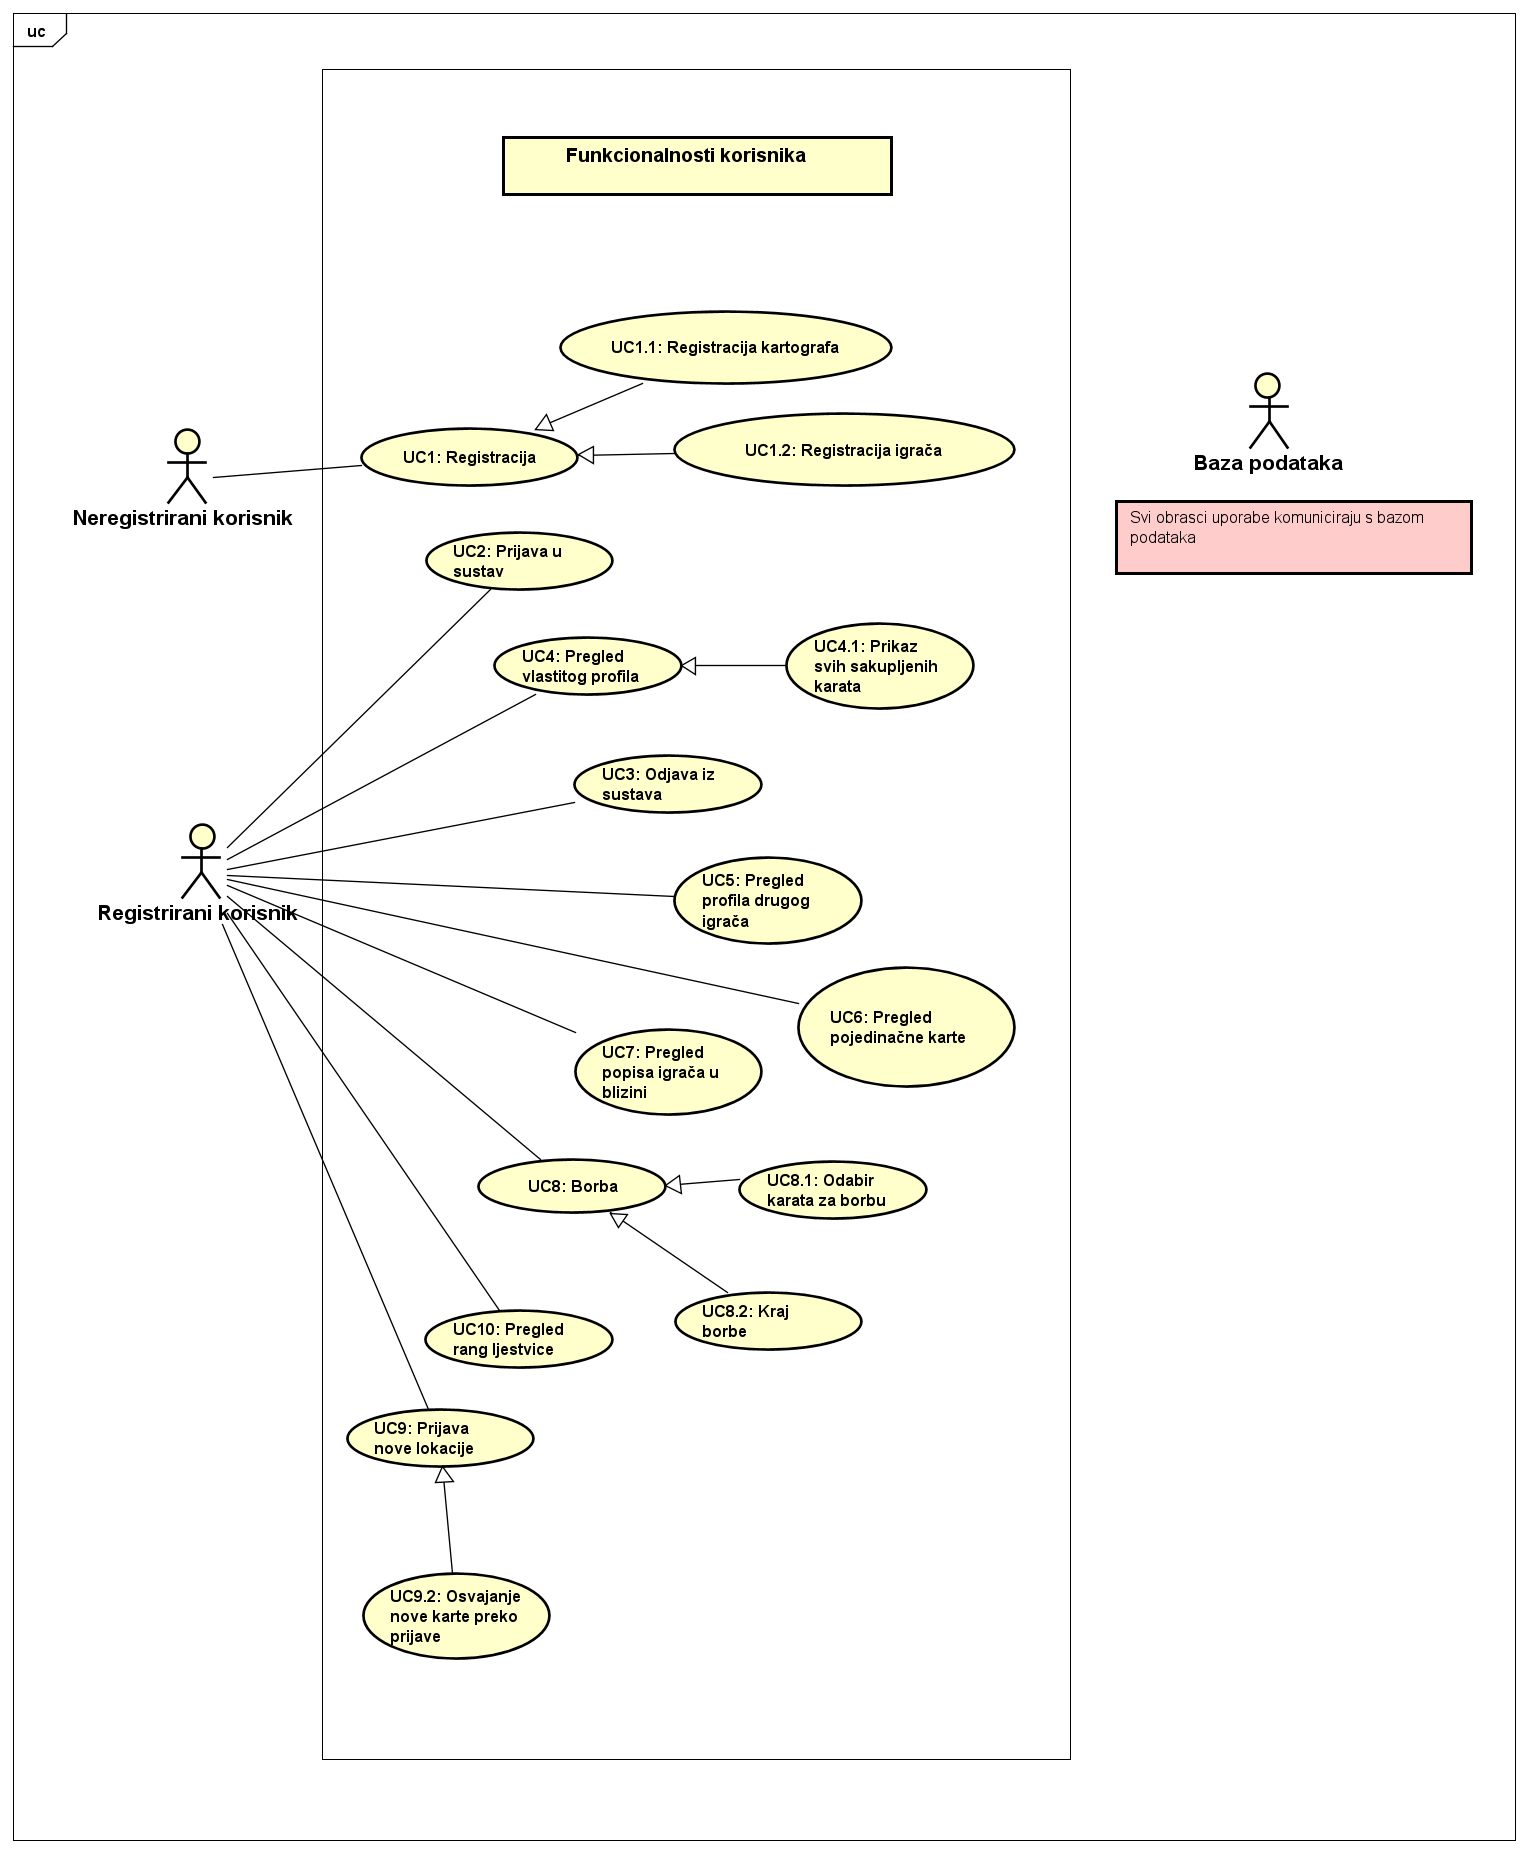
\includegraphics[scale=0.42]{dijagrami/funkcionalnosti_korisnika} \\
					\caption{Dijagram obrasca uporabe, funkcionalnosti neregistriranog i registriranog korisnika}
					\label{fig:funkcionalnosti_korisnika}
				\end{figure}
			
			\begin{figure}[H]
				\centering
				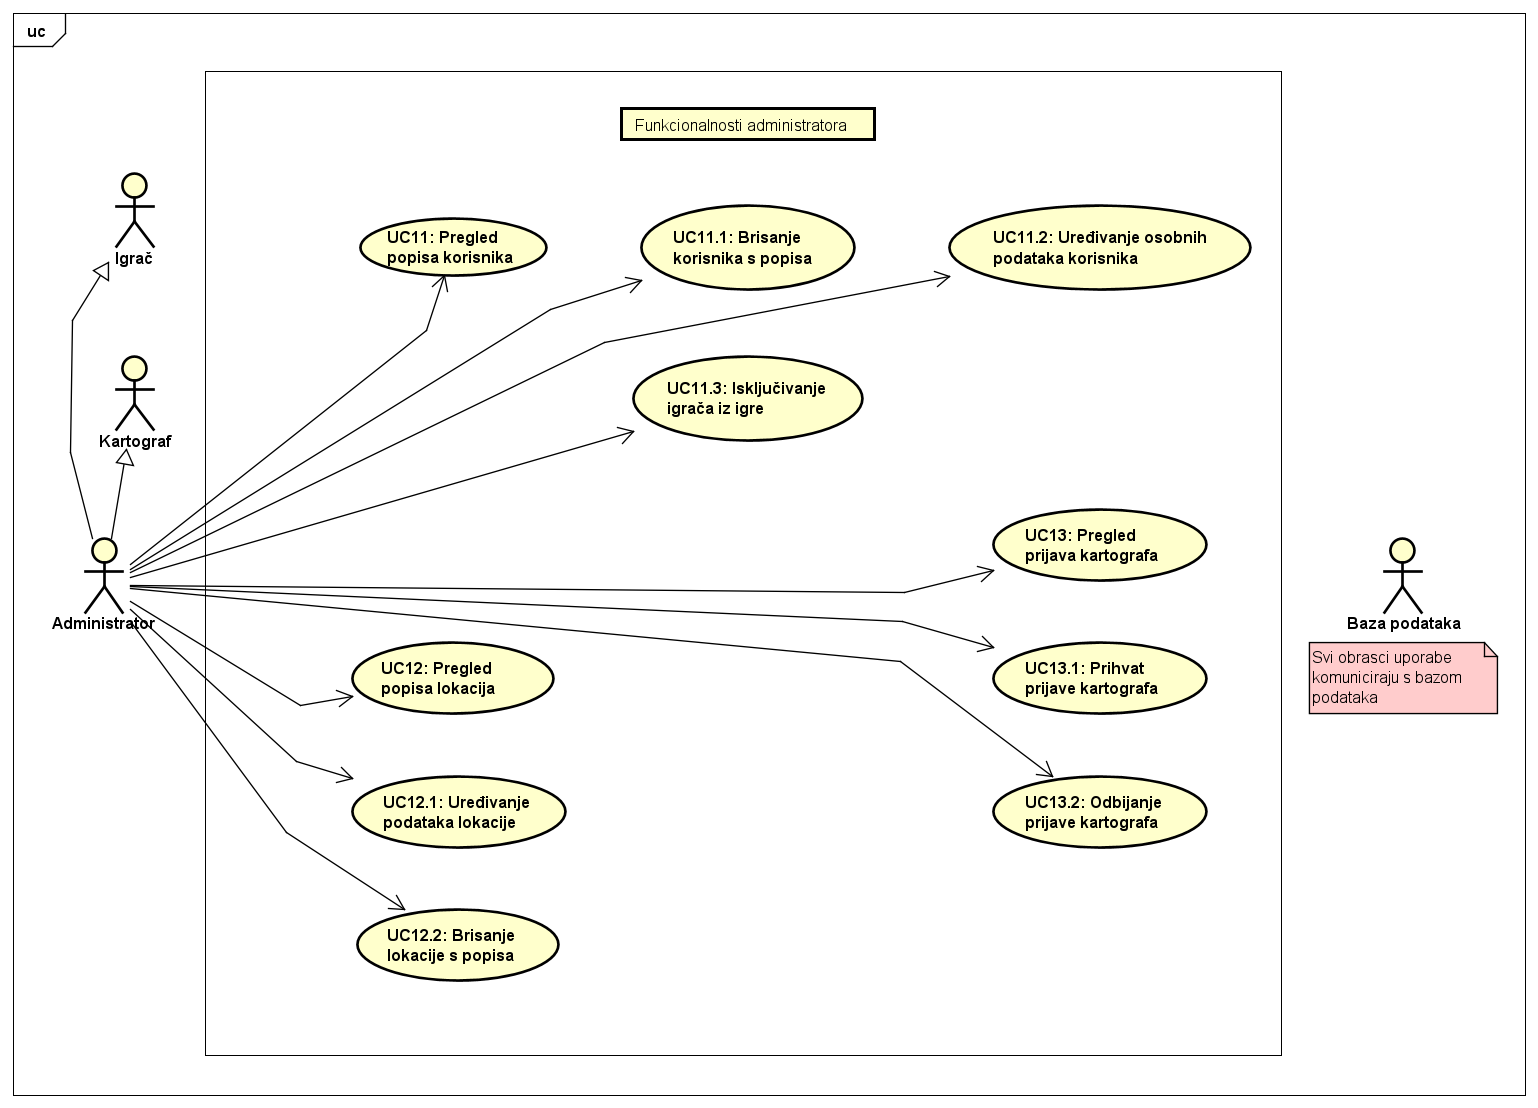
\includegraphics[scale=0.42]{dijagrami/funkcionalnosti_administratora} \\
				\caption{Dijagram obrasca uporabe, funkcionalnosti administratora}
				\label{fig:funkcionalnosti_administratora} 
			\end{figure}
		
		\begin{figure}[H]
			\centering
			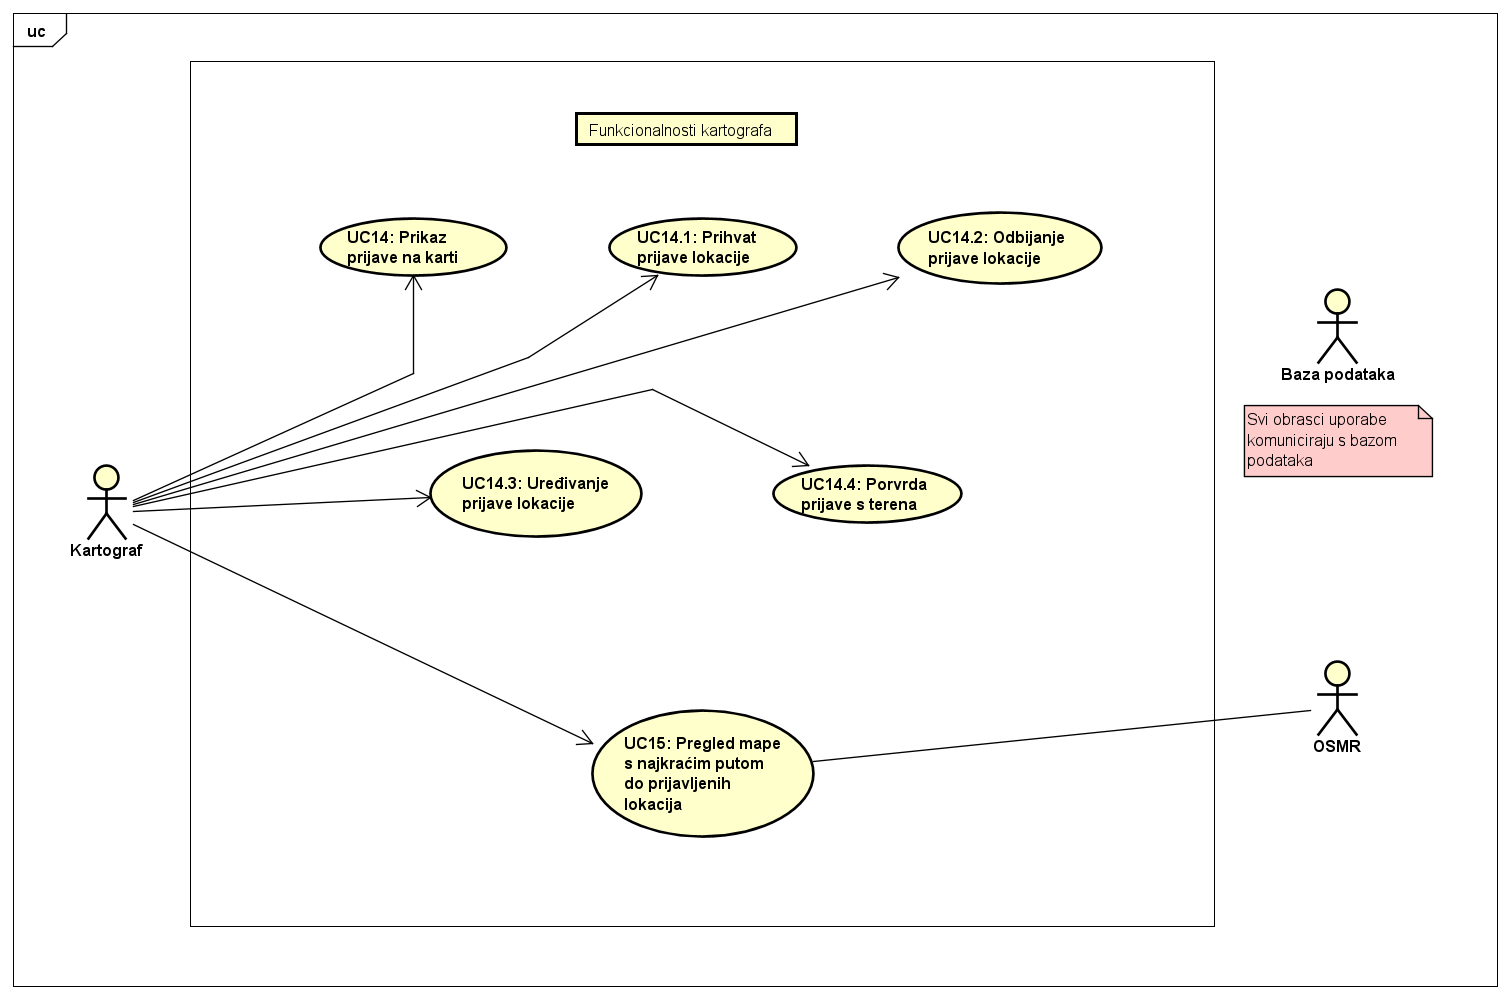
\includegraphics[scale=0.42]{dijagrami/funkcionalnosti_kartografa} \\
			\caption{Dijagram obrasca uporabe, funkcionalnosti kartografa}
			\label{fig:funkcionalnosti_kartografa} 
		\end{figure}
			\subsection{Sekvencijski dijagrami}
				
				\textbf{\textit{dio 1. revizije}}\\
				
				\textit{Nacrtati sekvencijske dijagrame koji modeliraju najvažnije dijelove sustava (max. 4 dijagrama). Ukoliko postoji nedoumica oko odabira, razjasniti s asistentom. Uz svaki dijagram napisati detaljni opis dijagrama.}
				\eject
	
		\section{Ostali zahtjevi}
		
			\textbf{\textit{dio 1. revizije}}\\
		 
			 \textit{Nefunkcionalni zahtjevi i zahtjevi domene primjene dopunjuju funkcionalne zahtjeve. Oni opisuju \textbf{kako se sustav treba ponašati} i koja \textbf{ograničenja} treba poštivati (performanse, korisničko iskustvo, pouzdanost, standardi kvalitete, sigurnost...). Primjeri takvih zahtjeva u Vašem projektu mogu biti: podržani jezici korisničkog sučelja, vrijeme odziva, najveći mogući podržani broj korisnika, podržane web/mobilne platforme, razina zaštite (protokoli komunikacije, kriptiranje...)... Svaki takav zahtjev potrebno je navesti u jednoj ili dvije rečenice.}
			 
			 
			 
	